\documentclass[xcolor=svgnames,handout,aspectratio=169]{beamer}

\usepackage[utf8]    {inputenc}
\usepackage[T1]      {fontenc}
\usepackage[english] {babel}

\usepackage{amsmath,amsfonts,graphicx}
\usepackage{beamerleanprogress}
\usepackage{media9}

\usepackage{tikz}
\usetikzlibrary{shapes,arrows}

\title
  [Short Title\hspace{2em}]
  {Smarter Smartmirror}

\author
  [Tobias Weis]
  {Tobias Weis}

\date
  {May 20, 2017}

\institute
  {Systems Engineering}


\begin{document}

\maketitle

\section{Introduction}
\title[Intro]{Introduction}

\begin{frame}
	\title[Intro]{Introduction}

  Building a smarter Smartmirror

  \begin{itemize}
  \item Smarter Smartmirror
  \item Requirements
  \item Hardware
  \item Software
  \end{itemize}
\end{frame}

\begin{frame}
	{Smarter Smartmirror}
	\begin{tabular}{cl}  
         \begin{tabular}{c}
           %\includegraphics[height=5cm, width=3.5cm]{horner}
           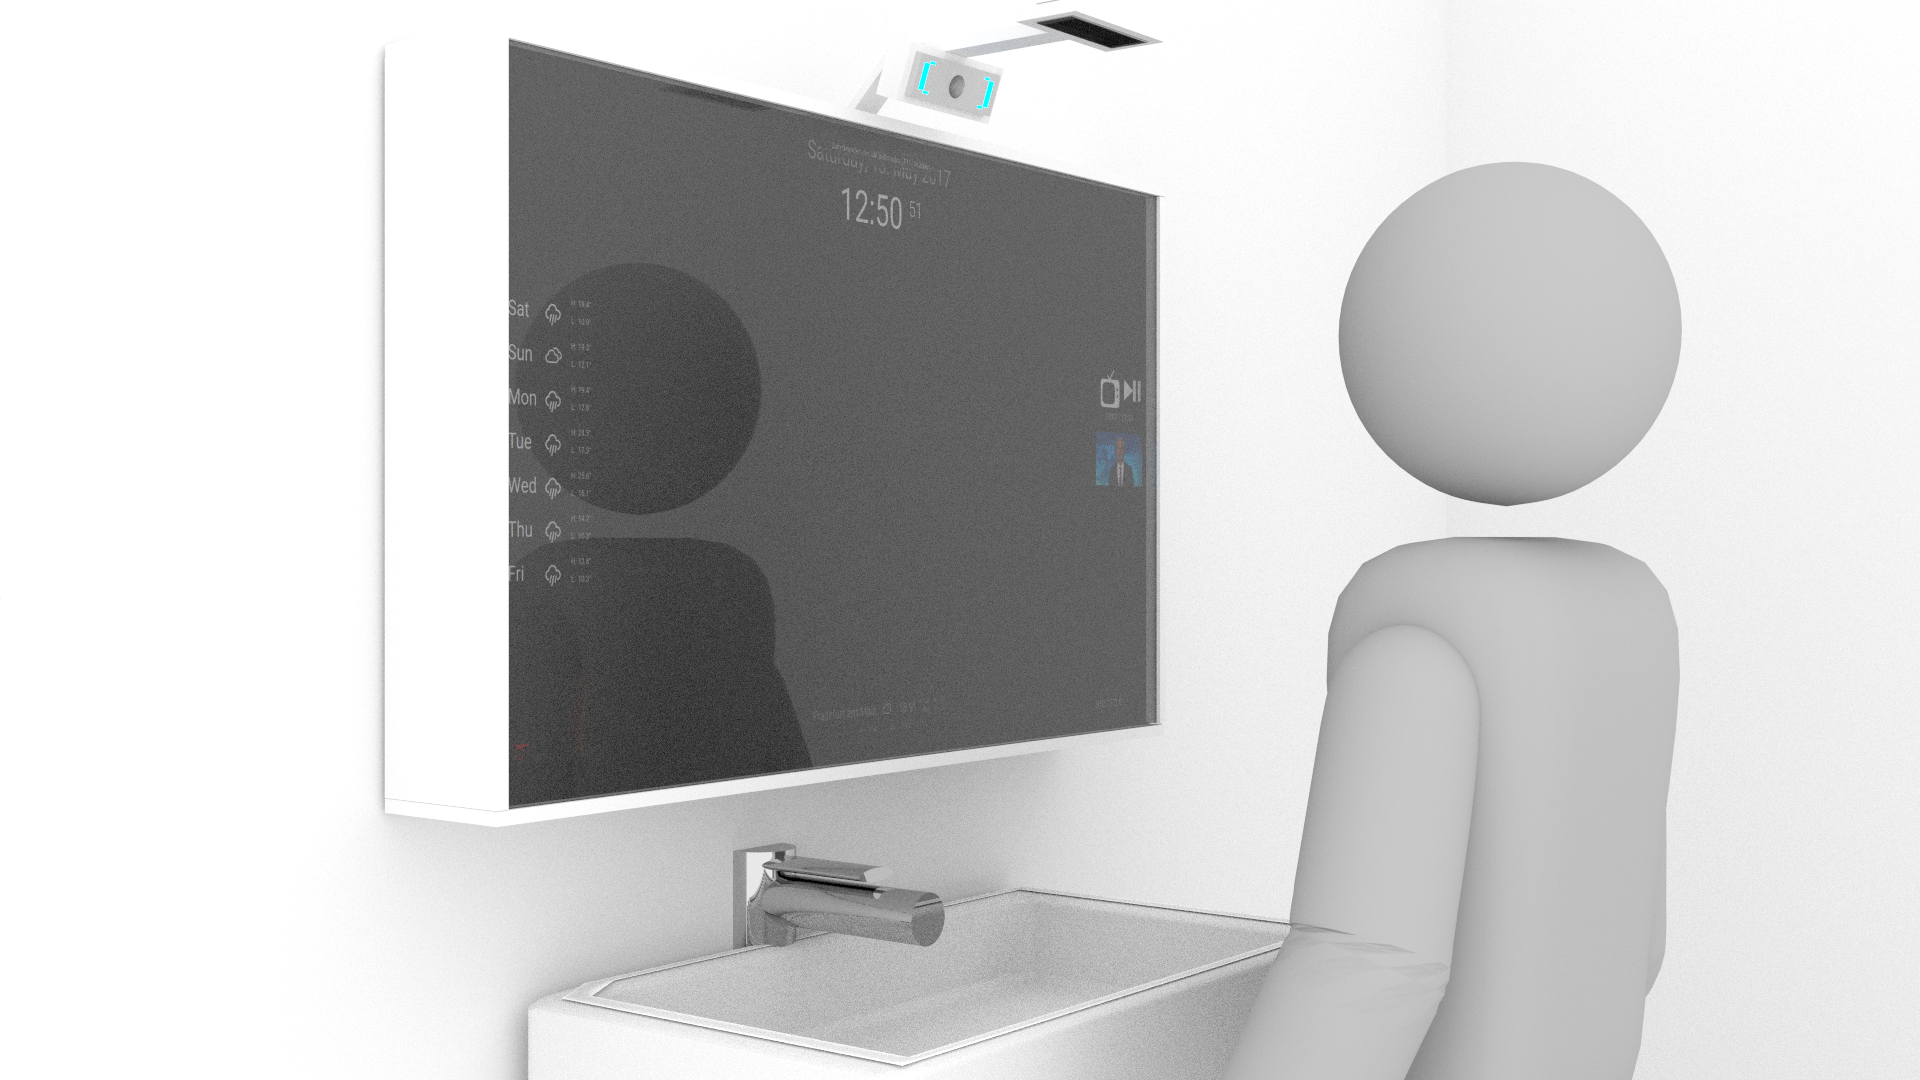
\includegraphics[width=.5\linewidth]{images/mirror_complete}
           \end{tabular}
           & \begin{tabular}{l}
             \parbox{0.4\linewidth}{%  change the parbox width as appropiate
             \textbf{Motivation:} Satisfy daily need of information in an unobtrusive way,
             without holding a device or sacrificing time:
			 Extend the bathroom mirror to both mirror your face and display information!
             While brushing the teeth you cannot do anything else anyway!
    		}
         \end{tabular}  \\
	\end{tabular}
\end{frame}

\section{Requirements}
\title[Requirements]{Requirements}

\begin{frame}
	{Requirements}
	\textbf{General}
	\begin{itemize}
		\item Mirror your face
	\end{itemize}
	\vspace{5mm}

	\textbf{Information needs}
	\begin{itemize}
		\item Time
		\item Weather
		\item News
		\item Calendar
		\item Stock prices
	\end{itemize}
	
	\vspace{5mm}
	
	\textbf{Usability}
	\begin{itemize}
		\item Easy control without touching the mirror
		\item Play video news (max. 5 minutes)
		\item Identify users to provide personalized information
	\end{itemize}
\end{frame}

\begin{frame}
	{Mirror}
	How to display information and still be a mirror?\\
	Two-way mirrors allow light from the backside to pass through:\\
	\vspace{0.5cm}
	\hspace{1cm} Regular mirror \hspace{5cm} Two-way mirror
	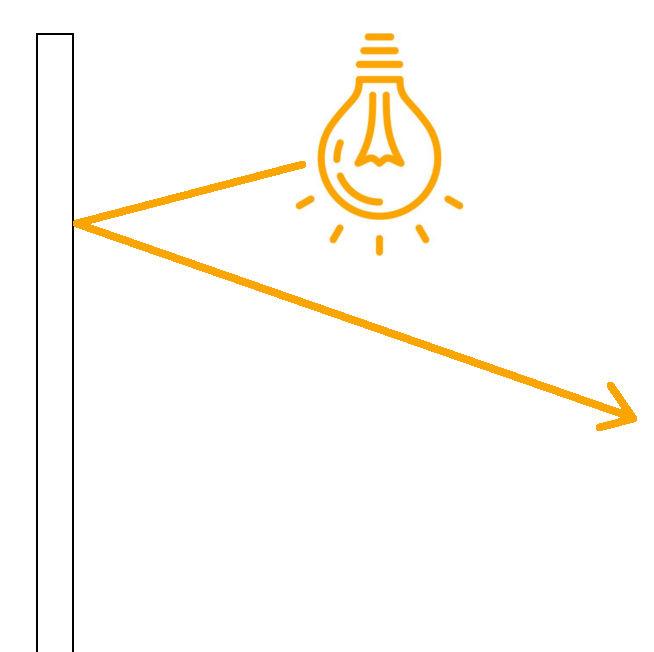
\includegraphics[height=4.5cm]{images/smartmirror_principle.png}
	\hspace{1.5cm}
	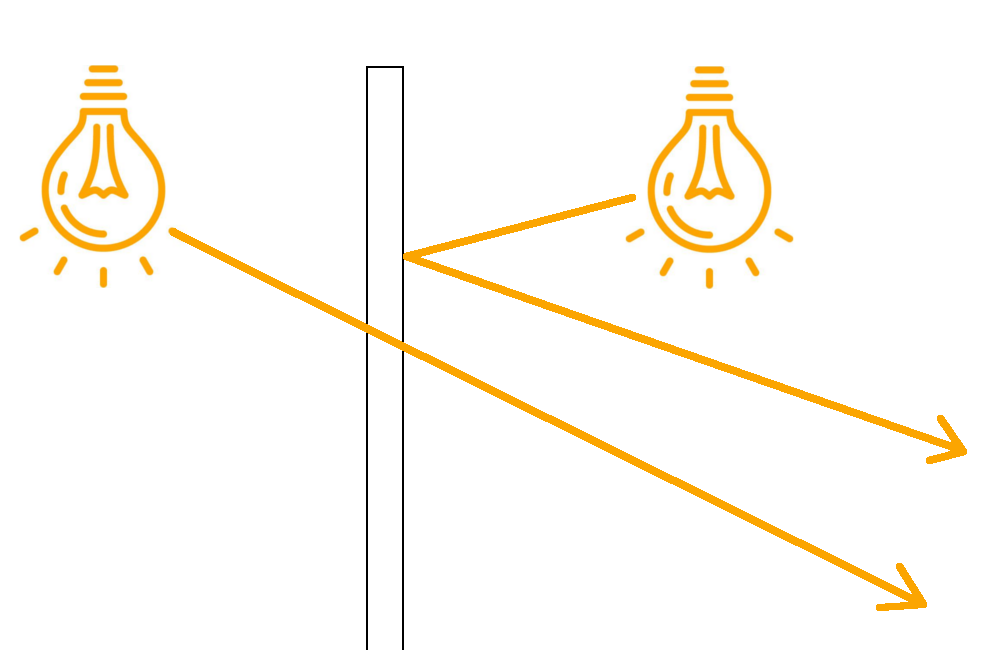
\includegraphics[height=4.5cm]{images/smartmirror_principle_2.png}
\end{frame}

\begin{frame}
	{Requirement mapping}
	
	\begin{tabular}{cl}  
			\parbox{0.6\linewidth}{
				\textbf{Sources of required information}
				\begin{itemize}
					\item Time - System time (works b/c of internet)
					\item Weather - Online service (JSON)
					\item News - Video (download using wget, script)
					\item Calendar - Google (JSON)
					\item Stock prices - Online service (JSON)
				\end{itemize}
				
				\textbf{Fetching and displaying}
				\begin{itemize}
					\item update each second
					\item simple markup to design display
					\item handle JSON data
					\item call system functions
					\item provide means of control 
				\end{itemize}
			}
		&
			\parbox{0.4\linewidth}{
				$\rightarrow$ Display as website in a browser in kiosk-mode
			}
	\end{tabular}
\end{frame}

\begin{frame}
	{Requirement mapping}
	\begin{tabular}{cl}  
			\parbox{0.6\linewidth}{
				\textbf{Usability}
				\begin{itemize}
					\item Control without touching
					\item Identify users
					\item Play videos
				\end{itemize}
			}
		&
			\parbox{0.4\linewidth}{
				$\rightarrow$ LeapMotion controller\\
				$\rightarrow$ Speech recognition\\
				$\rightarrow$ Facedetection $\rightarrow$ Camera\\
				$\rightarrow$ HTML 5 (mp4-video)\\
				$\rightarrow$ Sound output $\rightarrow$ Speakers
			}
	\end{tabular}	
\end{frame}


\section{Hardware}
\title[Hardware]{Hardware}

\begin{frame}
	{Requirement-mapping: Hardware}
	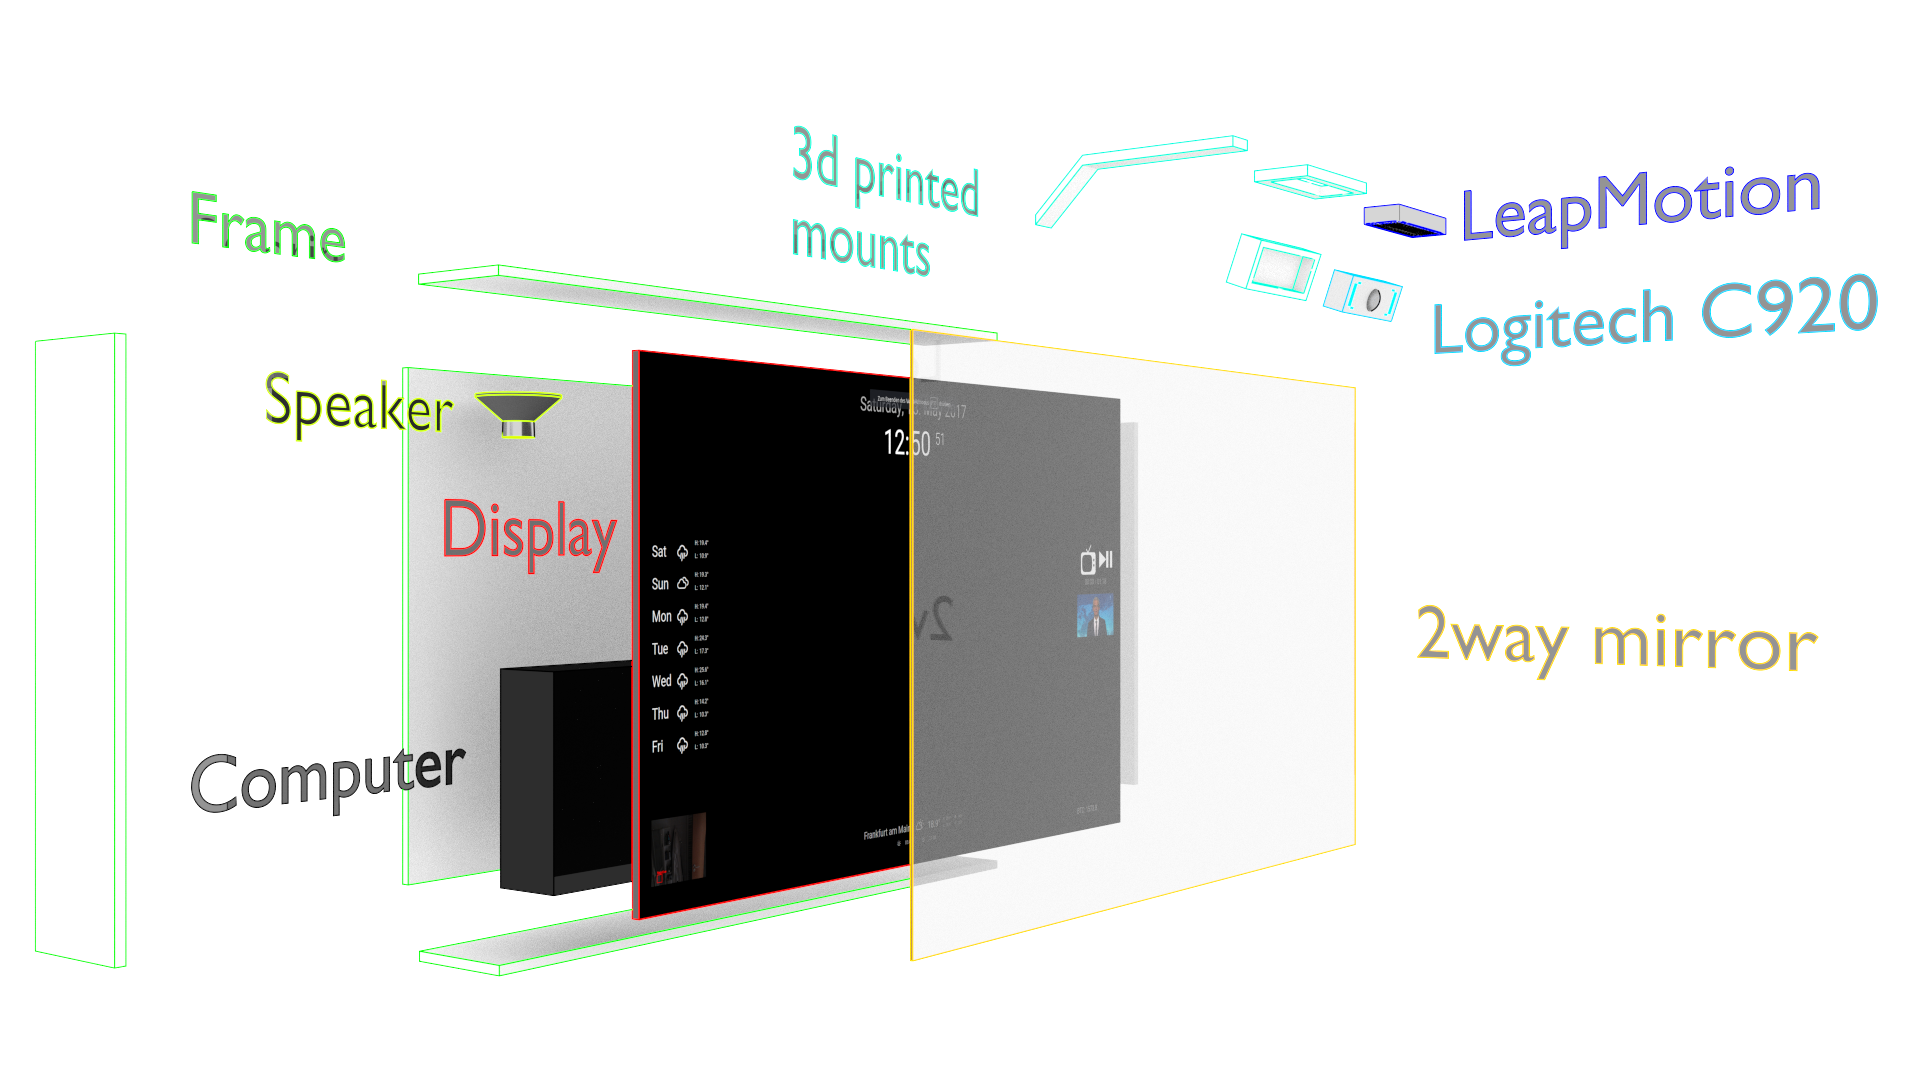
\includegraphics[width=\linewidth]{images/mirror_split_color}
\end{frame}


\section{Software}
\title[Software]{Software}

\begin{frame}
	{Software - GUI}
	\begin{tabular}{cl}  
			\parbox{0.35\linewidth}{
				\begin{itemize}
					\item HTML 5 website
					\item Browser in kiosk mode
					\item javascript modules
					\item control: keypresses
				\end{itemize}
			}&
			\parbox{0.6\linewidth}{			
				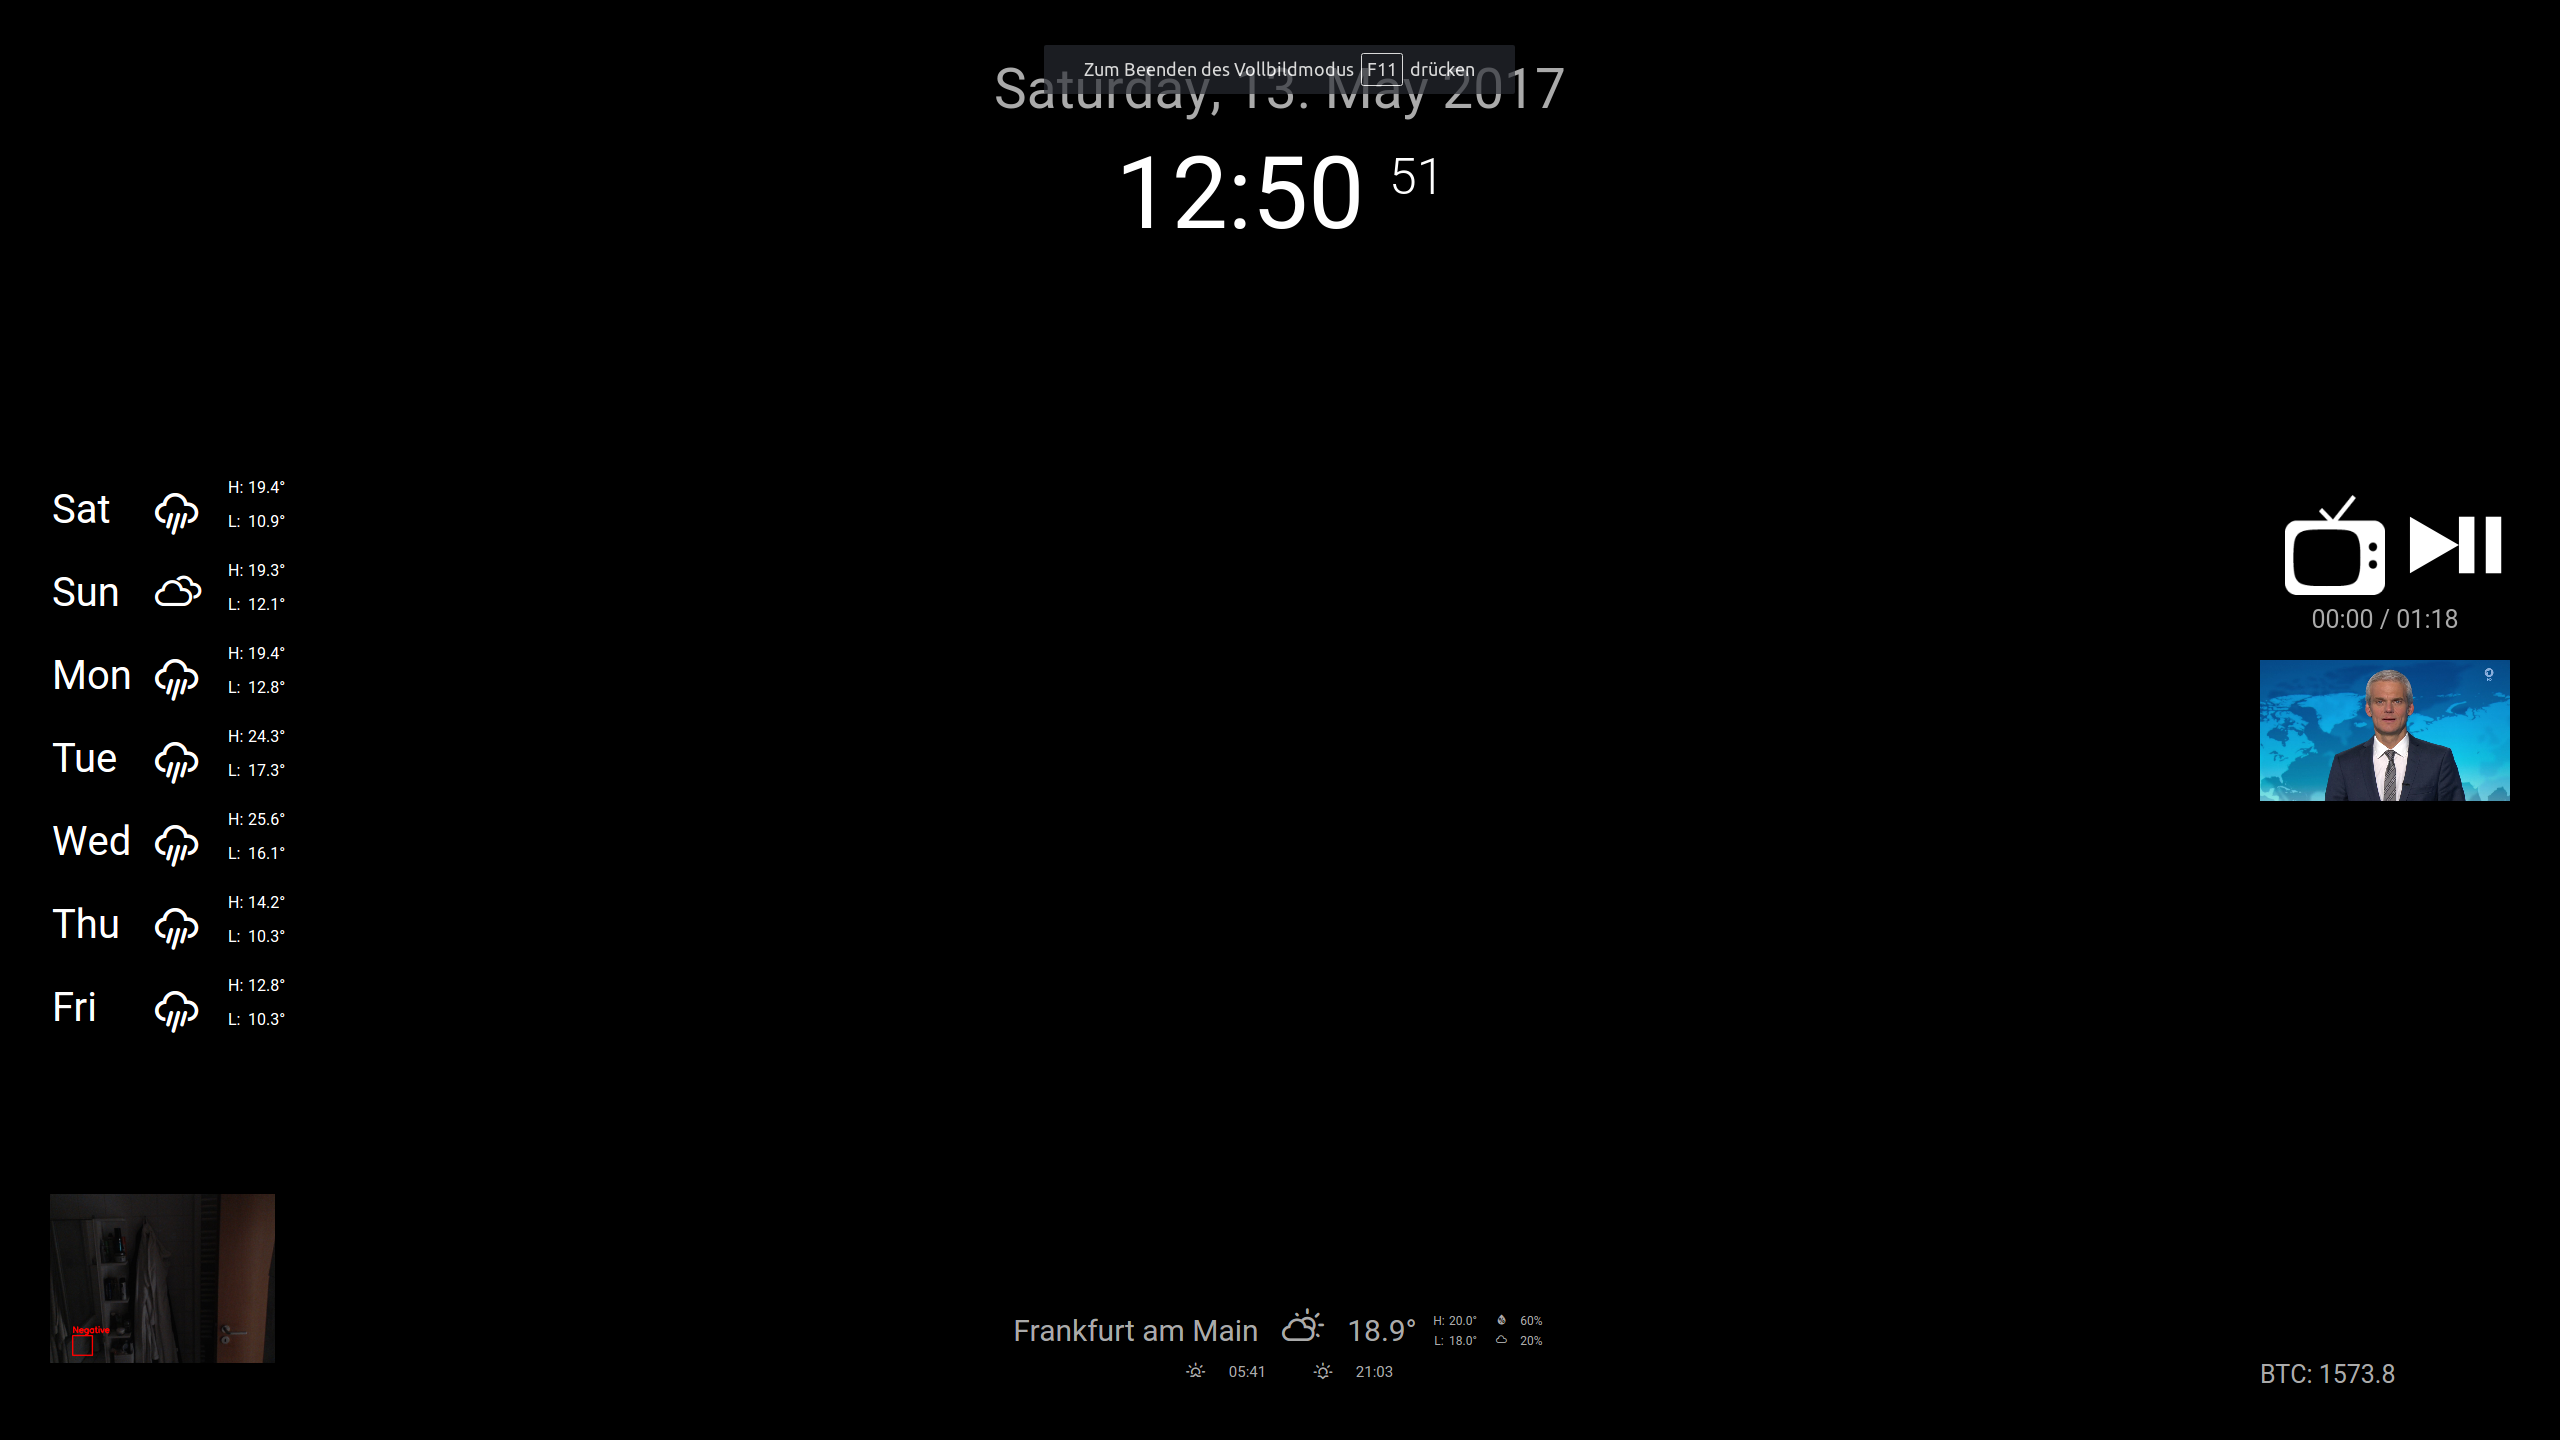
\includegraphics[width=\linewidth]{images/gui.png}
			}
		\end{tabular}
\end{frame}

\begin{frame}
	{Software - Control}

	\begin{tabular}{cl}  
			\parbox{0.35\linewidth}{
				\begin{itemize}
					\item Leap motion SDK (python)
					\item detect gestures
					\item map to keypresses (xdotool)
				\end{itemize}
				
				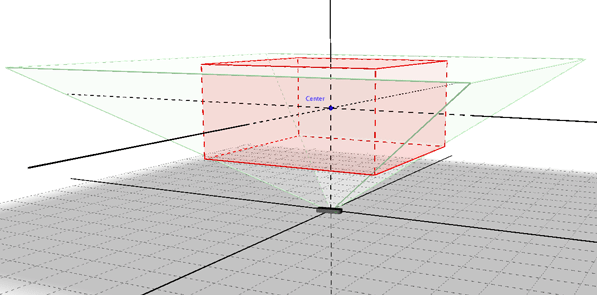
\includegraphics[width=\linewidth]{images/Leap_InteractionBox}
			}&
			\parbox{0.6\linewidth}{			
				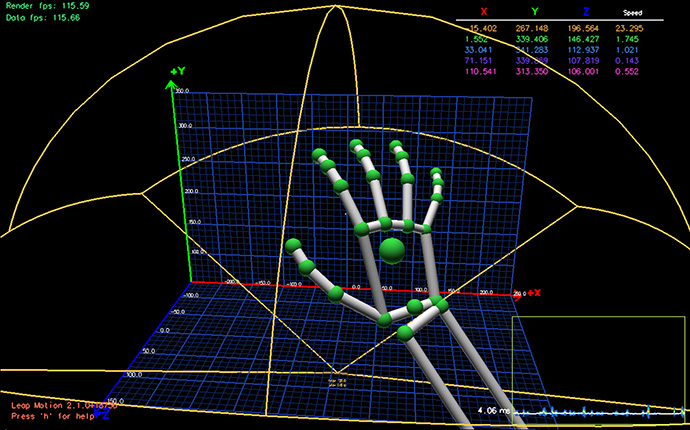
\includegraphics[width=\linewidth]{images/leap_visualizer.jpg}
			}
		\end{tabular}
\end{frame}

\begin{frame}
	{Software - Control}

	\begin{tabular}{cl} 
			\parbox{0.7\linewidth}{
				\textbf{Leap motion - specifics}
				\begin{itemize}
					\item Gesture recognition not reliable:\\
					Resort to \textit{coarse} gestures - whole hand movement,\\
					This results in a limited set of possible commands
				\end{itemize}
				
			}&
			\parbox{0.25\linewidth}{			
				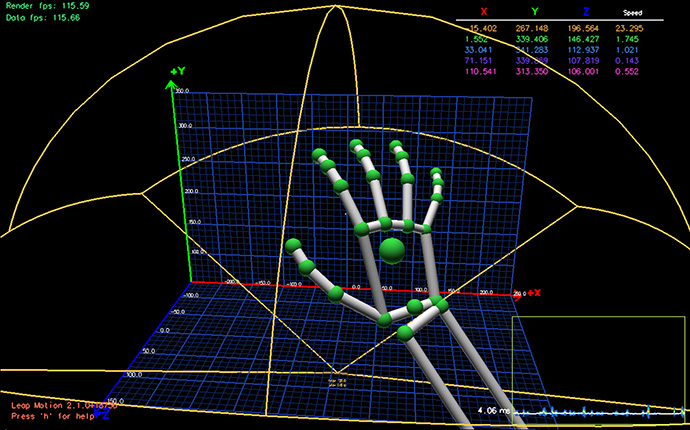
\includegraphics[width=\linewidth]{images/leap_visualizer.jpg}\\
				\vspace{5mm}
				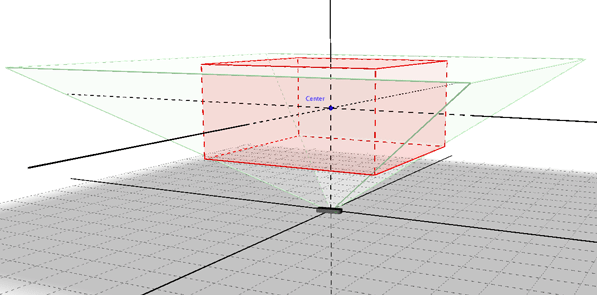
\includegraphics[width=\linewidth]{images/Leap_InteractionBox}				
			}
		\end{tabular}
\end{frame}


\begin{frame}
	{Software - Control}

	\begin{tabular}{cl}  
			\parbox{0.35\linewidth}{
				\begin{itemize}
					\item Voice recognition
					\item CMU pocketsphinx (python)
					\item map to keypresses (xdotool)
				\end{itemize}
			}&
			\parbox{0.6\linewidth}{			
				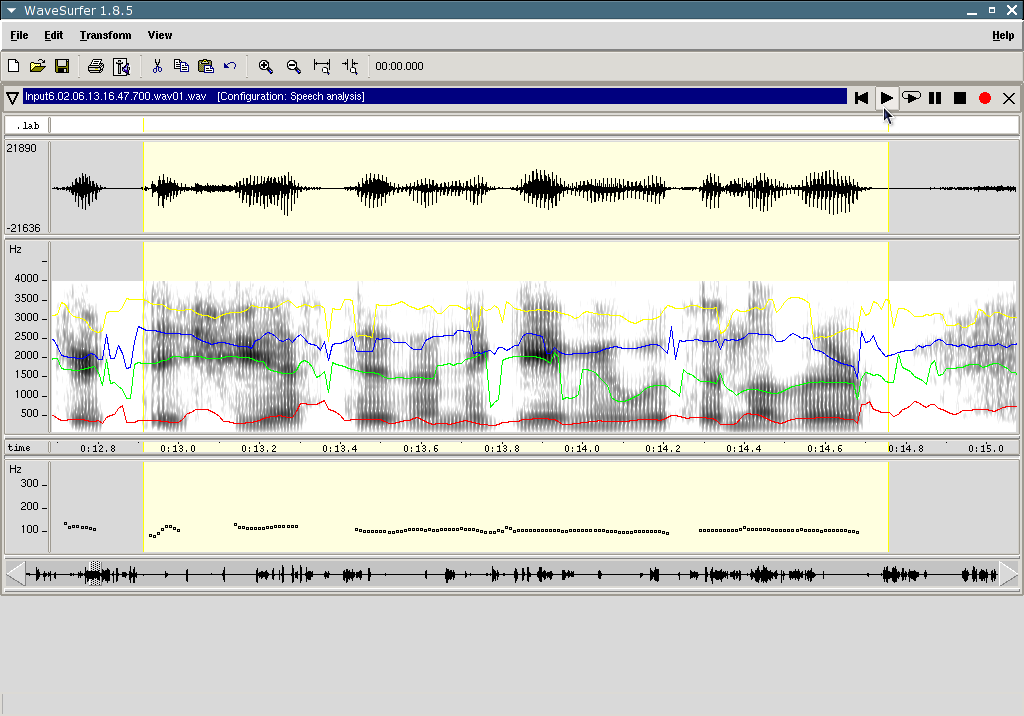
\includegraphics[width=\linewidth]{images/waveform}
			}
		\end{tabular}
\end{frame}


\begin{frame}
	{Software - Control}

	\begin{tabular}{cl}  
			\parbox{0.7\linewidth}{
				\textbf{Voice recognition specifics}
				\begin{itemize}
					\item Voice recognition has a lot of false detections out of the box:\\
						Build a knowledgebase from a custom phrase-dictionary,\\
						this improves accuracy a lot!
					\item Fails if video or music play
					\item Addition of new commands requires recompilation of knowledgebase
				\end{itemize}
			}&
			\parbox{0.25\linewidth}{			
				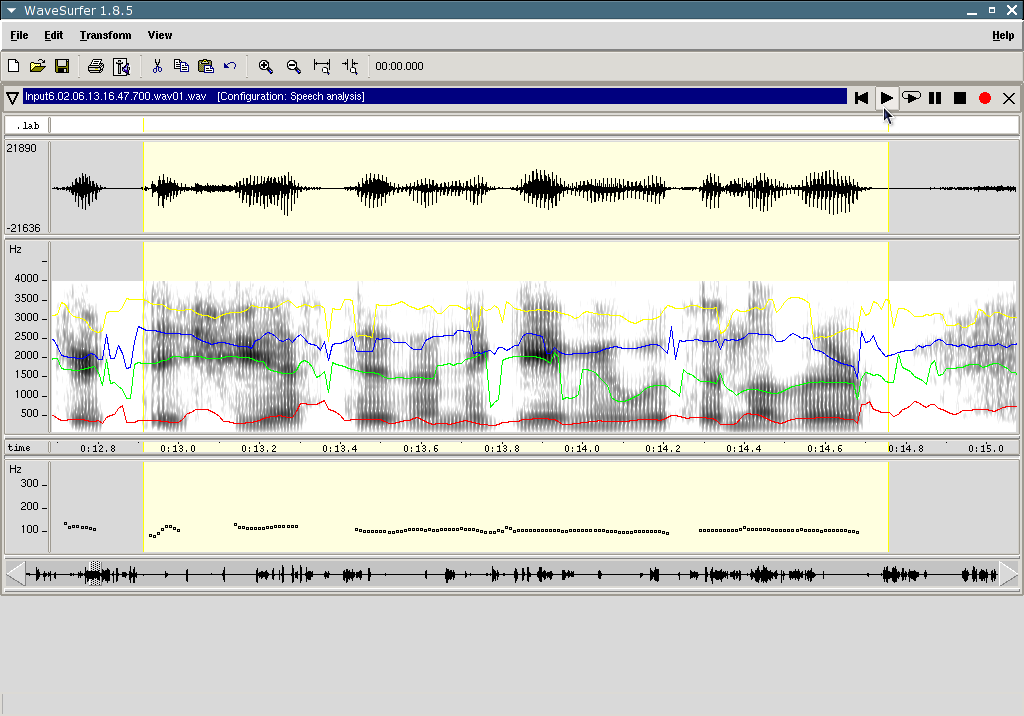
\includegraphics[width=\linewidth]{images/waveform}
			}
		\end{tabular}
\end{frame}


\begin{frame}
	{Software - Identify users}
	
		\begin{tabular}{cl}  
			\parbox{0.35\linewidth}{
				Extrinsic and intrinsic parameters of camera,
				as well as the layout of the room dictate
				the possible distance of the user to the sensor,
				and therefore the possible scalings.
			}&
			\parbox{0.6\linewidth}{			
				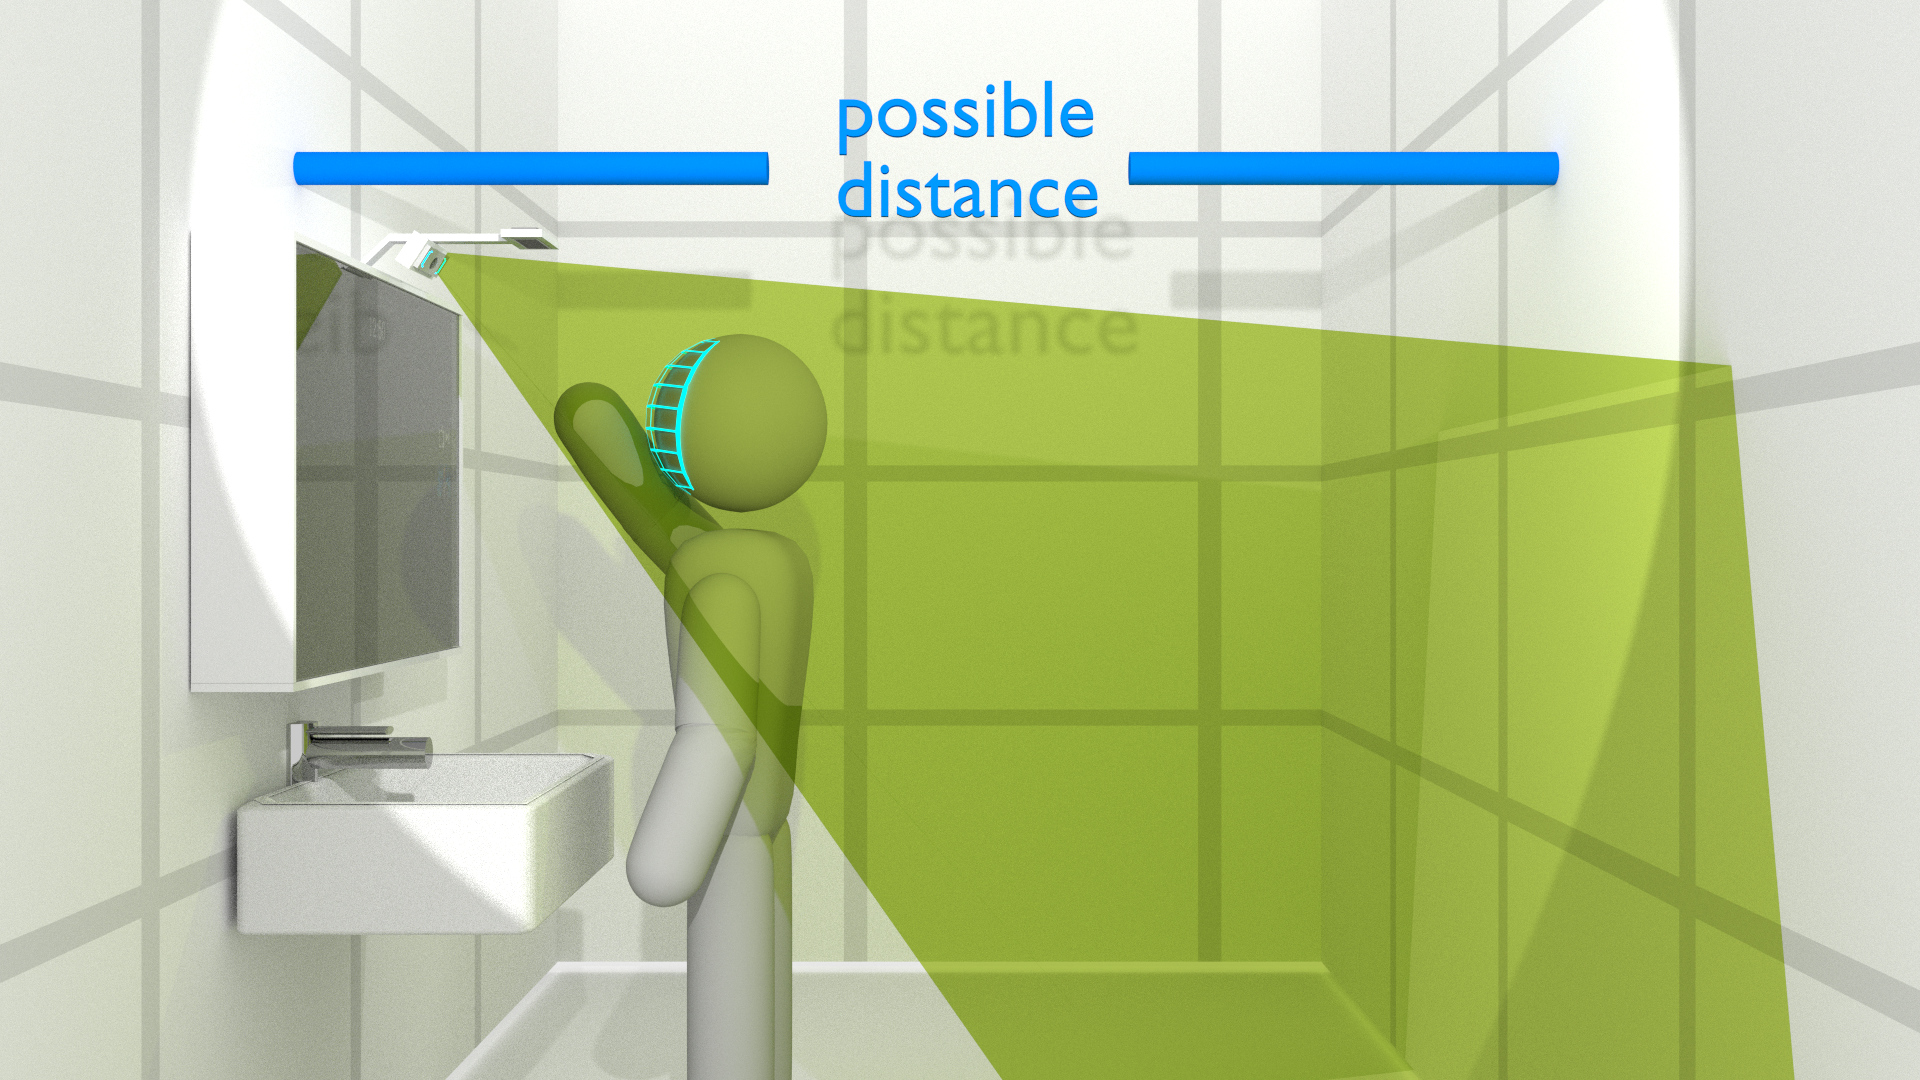
\includegraphics[width=\linewidth]{images/mirror_distance}
			}
		\end{tabular}

\end{frame}

\begin{frame}
	{Software - Identify users - Flowgraph}
	
	Constrained scaling: Pre-trained Haar-Cascade face-detector
	
%\tikzstyle{decision} = [diamond, draw, fill=blue!20, 
%    text width=4.5em, text badly centered, node distance=3cm, inner sep=0pt]
\tikzstyle{block} = [rectangle, draw, text width=5em, text centered, rounded corners]
\tikzstyle{line} = [draw, -latex']
\tikzstyle{cloud} = [draw, ellipse, minimum height=2em, text width=7em]
\center    
\begin{tikzpicture}[node distance = 4cm, auto,thick,scale=0.6, every node/.style={scale=0.6}]
    % Place nodes
    \node [block] (inp) {Picture stream};

    \node [cloud, right of=inp] (facedet) {Face detection (Haar Cascade)};
    
    \node [block, right of=facedet] (faces) {Face candidates (Patches)};
    
    \node [cloud, right of=faces] (recog) {Face recognition (CNN)};
    
    \node [block, right of=recog] (ident) {Identity estimate};
    
    % Draw edges
    \path [line] (inp) -- (facedet);
    \path [line] (facedet) -- (faces);
    \path [line] (faces) -- (recog);
    \path [line] (recog) -- (ident);
    %\path [line] (update) |- (identify);
    %\path [line] (decide) -- node {no}(stop);

    %\path [line,dashed] (system) -- (init);
    %\path [line,dashed] (system) |- (evaluate);
\end{tikzpicture}	
\end{frame}

\begin{frame}
	{Software - Identify users}

	\begin{tabular}{cl}  
			\parbox{0.4\linewidth}{			
				\textbf{Training efforts}
				\begin{itemize}
					\item Detect \& save face patches
					\item First few hundred images: manual classification\\
					afterwards semi-automatic (only correct errors)
					
					\item Train \& evaluate 3-layer CNN
				\end{itemize}
				\vspace{0.5cm}
				\begin{itemize}
					\item approx. 10k images/class
				\end{itemize}
			}&
			\parbox{0.55\linewidth}{			
				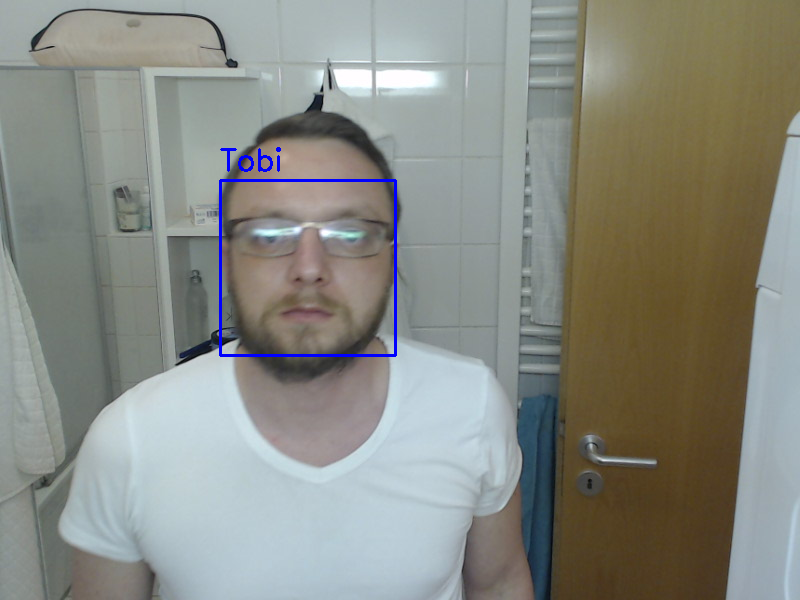
\includegraphics[width=\linewidth]{images/faceimg}
			}
		\end{tabular}
\end{frame}



\begin{frame}
	{Software - Identify users}
	\parbox{0.45\linewidth}{
	\begin{figure}
	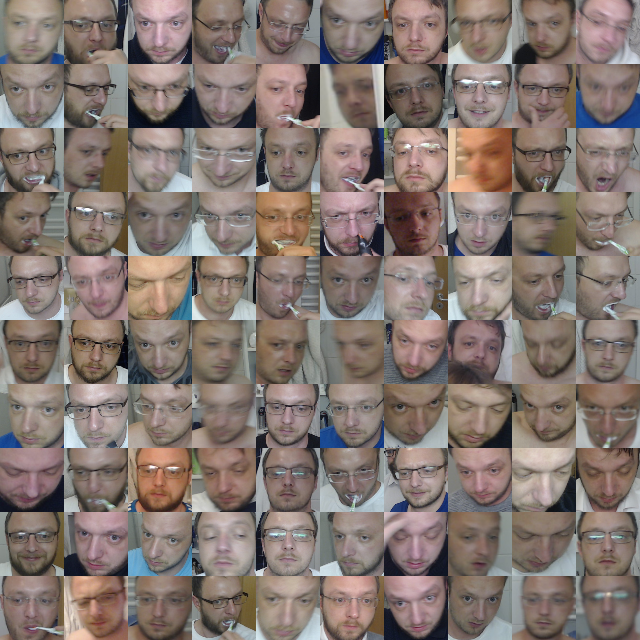
\includegraphics[width=\linewidth]{images/mosaic_tobi.png}
	\caption{Example trainingset Tobi}
	\end{figure}
	}
	\parbox{0.45\linewidth}{	
	\begin{figure}
	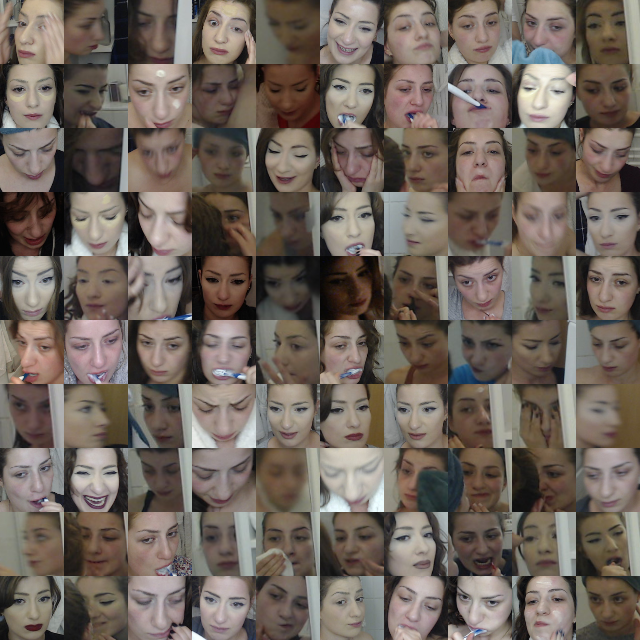
\includegraphics[width=\linewidth]{images/mosaic_mari.png}
	\caption{Example trainingset Mariam}	
	\end{figure}
	}
\end{frame}

\begin{frame}
	{Software - Identify users}
	\parbox{0.45\linewidth}{
	\begin{figure}
	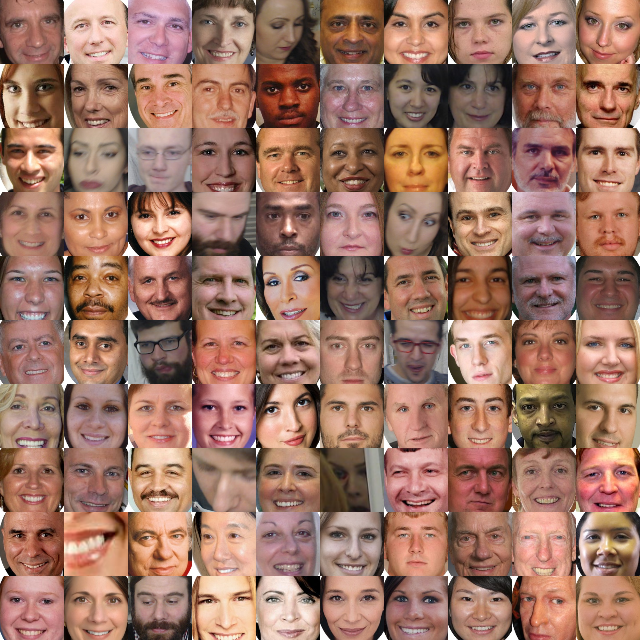
\includegraphics[width=\linewidth]{images/mosaic.png}
	\caption{Example trainingset Other}
	\end{figure}
	}
	\parbox{0.45\linewidth}{	
	\begin{figure}
	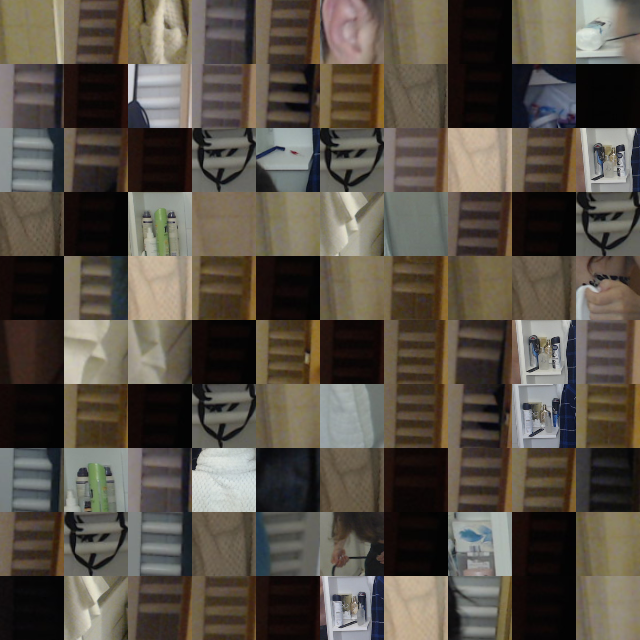
\includegraphics[width=\linewidth]{images/mosaic_negative.png}
	\caption{Example trainingset Negative}	
	\end{figure}
	}
\end{frame}


\section{System}
\title[System]{System}

\begin{frame}
	{System - Flowgraph}	
\tikzstyle{decision} = [diamond, draw, text width=4.5em, text badly centered, inner sep=0pt]
\usetikzlibrary{calc}
\usetikzlibrary{positioning}
\tikzstyle{block} = [rectangle, draw, text width=5em, text centered, rounded corners]
\tikzstyle{line} = [draw, -latex']
\tikzstyle{cloud} = [draw, ellipse, minimum height=2em, text width=7em]
\center    
\begin{tikzpicture}[node distance = 1cm, auto,thick,scale=0.5, every node/.style={scale=0.5}]
    % Place nodes
    \node [block] (motion) {Read motion detector};
    \node [decision, right=of motion] (motdet) {Motion?};
	\node [block, right=of motdet] (start) {Start timer};
	
	\node [block, above=of start] (screen) {Activate screen};
	
	\node [block, right=of start] (face) {Activate face recog};
	\node [block, below=of face] (voice) {Activate speech recog};
	\node [block, above=of face] (gesture) {Activate gesture recog};
		
	\node [block, right=of face] (keys) {Control-API};
	
	\node [block, right=of keys] (browser) {Browser};
	\node [block, right=of browser] (js_weather) {JS weather};
	\node [block, above=of js_weather] (js_time) {JS time};	
	\node [block, below=of js_weather] (js_stocks) {JS stocks};
	\node [block, above=of js_time] (js_video) {JS video};
	\node [block, below=of js_stocks] (js_calendar) {JS calendar};
	
	\node [block, above right=of gesture] (synth) {Speech synthesis};
	
	\path [line] (motion) -- (motdet);
	\path [line] (motdet) -- node[above,midway]{Yes} (start);
	\path[line] (motdet.south) |- node[above,right]{No} ($(motion.south) + (0., -1.)$) -- (motion.south) ;
	
	\path[line] (start) -- (screen);
	\path[line] (gesture) |- ($(gesture.north west) + (-0.5, 0.5)$) |- (gesture);
	\path[line] (voice) |- ($(voice.south west) + (-0.5, -0.5)$) |- (voice);
	\path[line] (face) |- ($(face.south west) + (-0.5, -0.5)$) |- (face);
		
	\path[line] (start) -- (voice);
	\path[line] (start) -- (face);
	
	\path[line,dashed] (voice) -- (keys);
	\path[line,dashed] (face) -- (keys);
	\path[line,dashed] (gesture) -- (keys);
	
	\path[line,dashed] (keys) -- (browser);
    %\path [line] (update) |- (identify);
    
    \path[line] (js_weather) -- (browser);
    \path[line] (js_time) -- (browser);
    \path[line] (js_stocks) -- (browser);
    \path[line] (js_video) -- (browser);
    \path[line] (browser) -- (js_video);
    \path[line] (browser) -- (js_calendar);
    \path[line] (js_calendar) -- (browser);
    
    \path[line] (gesture) -- (synth);
    \path[line] (face) -- (synth);

    %\path [line,dashed] (system) -- (init);
    %\path [line,dashed] (system) |- (evaluate);
\end{tikzpicture}	
\end{frame}

\begin{frame}
	{Result}
	\center
	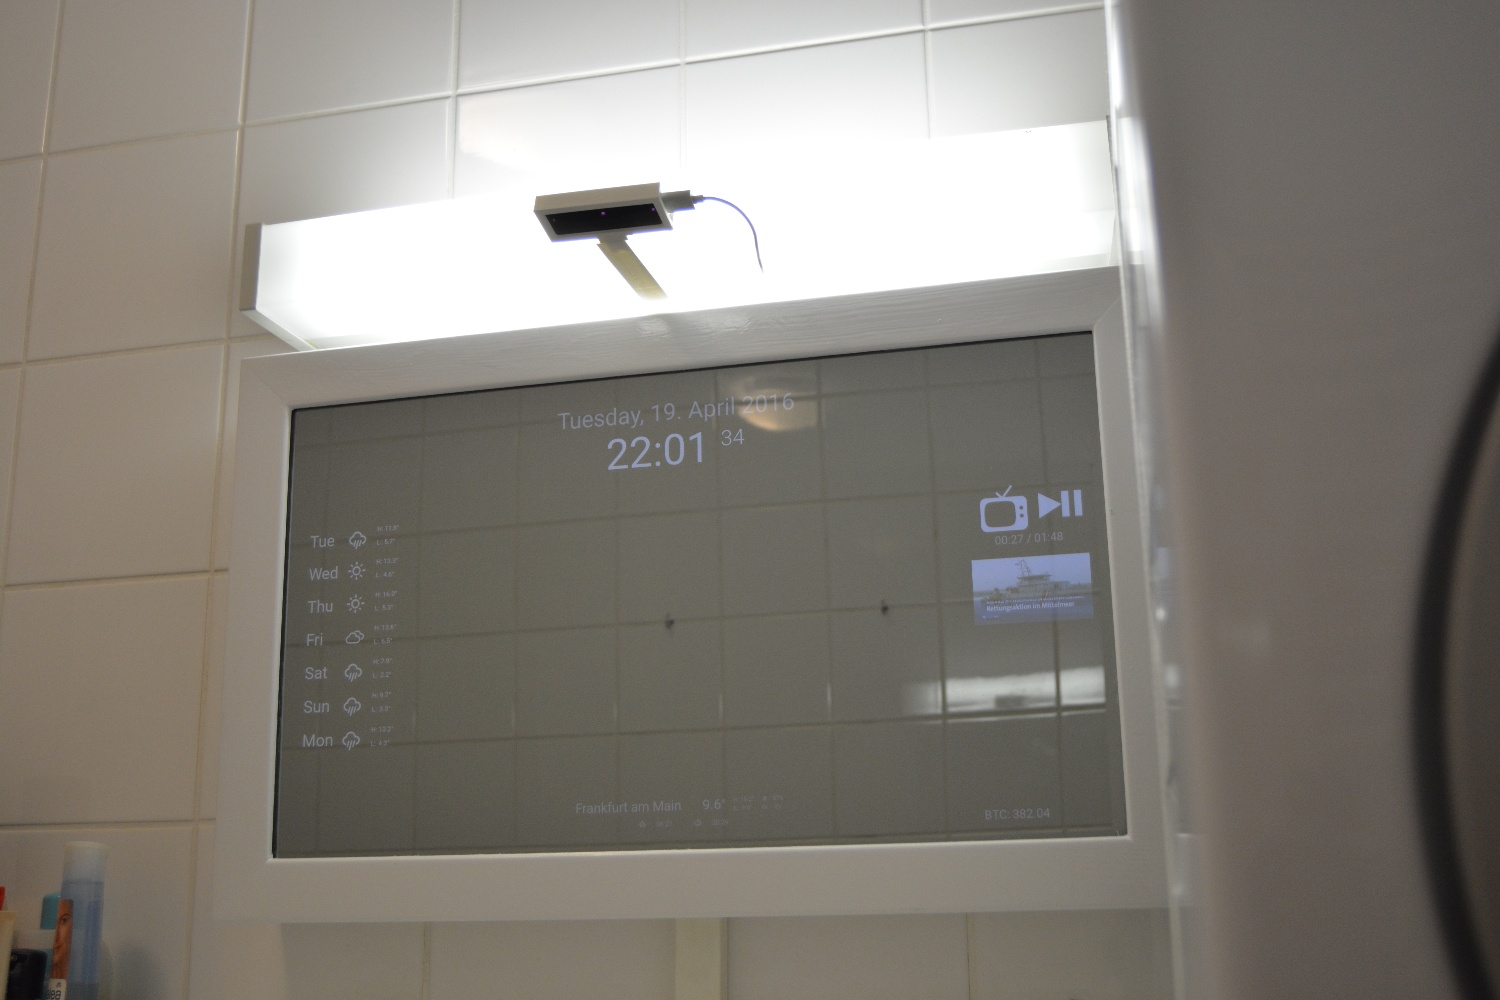
\includegraphics[width=.7\linewidth]{images/mirror_real}
\end{frame}

\begin{frame}
	{Science fiction}
	
	\begin{itemize}
		\item Cluster unknown faces and automatically retrain (e.g. recurring guests/friends)
		\item Non-invasive health diagnosis
		\item Selection of \emph{good} pictures to create a timelapse
		\item Personal metrics: create a journal of wakeup-times
		\item Personal assistant: voice-interaction (set reminders, detach early email, etc.)
		\item Interface with smart home: automatically start the coffee-brewer on wake-up
	\end{itemize}
\end{frame}


\begin{frame}
  {End}
	Some funny extensions
	\begin{itemize}
		\item Bloody Mary Protocol (Video)
	\end{itemize}

\end{frame}

%\begin{frame}
%  {Equations}
%
%  Equations are easy
%  \begin{itemize}
%  \item Just copy/paste equations\pause
%  \item From the paper!
%    \begin{equation*}
%      \textbf{p}^* = \underset{\textbf{p}}{\arg\!\min}~\sum_{\textbf{x}}\left[ I(\textbf{W}(\textbf{x};\textbf{p})) - T(\textbf{x}) \right]^2
%    \end{equation*}
%  \end{itemize}
%\end{frame}
%
%
%\begin{frame}
%  {Pictures}
%
%  \begin{figure}[t]
%    \centering
%    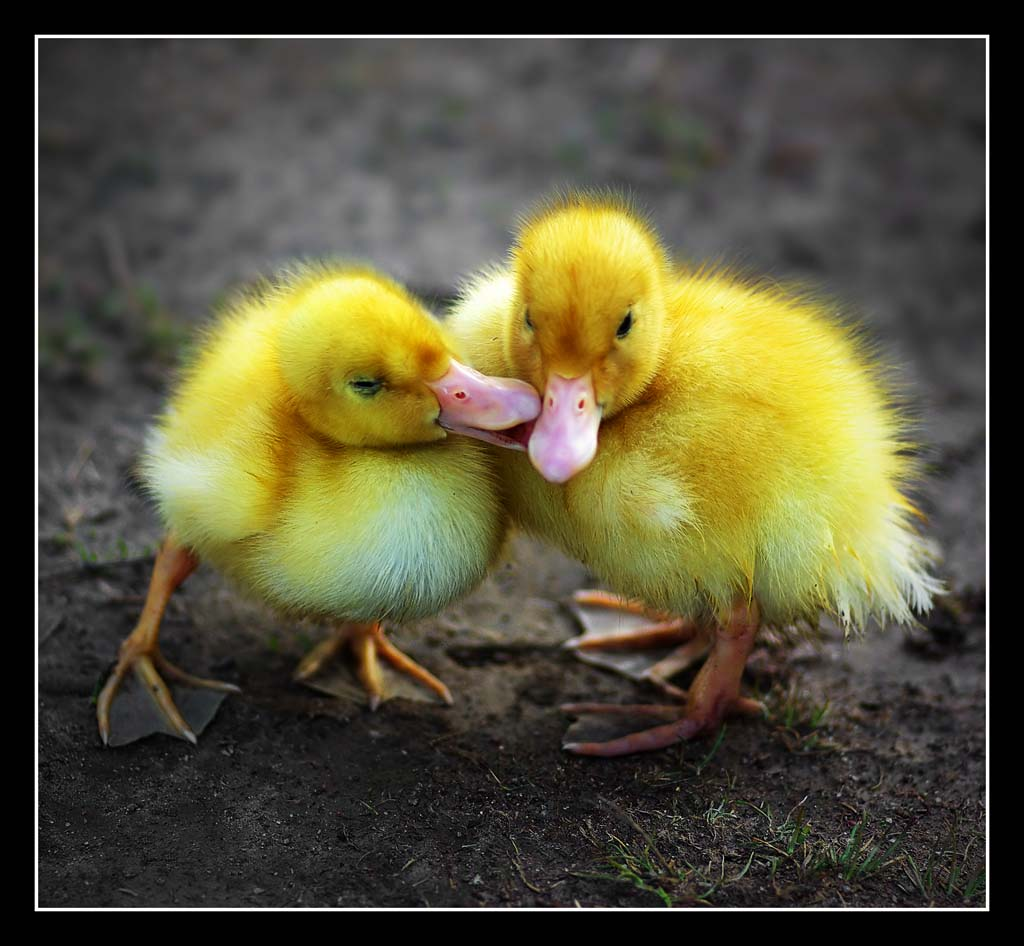
\includegraphics[height=\dimexpr11\textheight/16\relax]{ducks}
%    \caption{Kissing ducks}
%  \end{figure}
%\end{frame}
%
%
%\begin{frame}
%  {A Movie}
%
%  \begin{block}{Some block}
%    \begin{itemize}
%    \item Movies only seem to work in Adobe Reader
%    \item Movie file is not embedded, it must be on the computer
%    \end{itemize}
%  \end{block}
%
%  \begin{exampleblock}{Some more block}
%    Movies only seem to work in Adobe Reader\par
%    Movie file is not embedded, it must be on the computer
%  \end{exampleblock}
%
%  \begin{alertblock}{}
%    Some text in here.
%    \begin{itemize}
%    \item Movies only seem to work in Adobe Reader
%    \item Movie file is not embedded, it must be on the computer
%    \end{itemize}
%  \end{alertblock}
%\end{frame}
%
%
%
%\section
%  {Conclusion}
%
%\begin{frame}
%  {Credits}
%
%  \begin{itemize}
%  \item Brought to you by Cédric Mauclair
%  \item Please let me know about improvements!
%  \item inspiration: \url{http://www.shawnlankton.com}... (in code)
%  \end{itemize}
%\end{frame}

\end{document}

